\setkeys{Gin}{keepaspectratio}

\begin{figure*}[t]
\centering

\begin{tikzpicture}[
x=1cm,
y=1cm,
stage/.style={
    draw=gray!65,
    dashed,
    rounded corners=4pt,
    fill=gray!5,
    line width=0.3pt,
    inner sep=0pt
},
branch/.style={
    draw=gray!55,
    rounded corners=3pt,
    fill=white,
    line width=0.3pt,
    inner sep=0pt
},
paneltitle/.style={
    font=\bfseries\tiny,
    anchor=south west,
    inner sep=0pt
},
versionlabel/.style={
    font=\bfseries\tiny,
    anchor=south,
    inner sep=1pt
},
dots/.style={
    font=\bfseries\small,
    anchor=south,
    inner sep=1pt
},
img/.style={
    inner sep=0pt,
    outer sep=0pt,
    anchor=center
},
sourceimg/.style={
    draw=gray!45,
    line width=0.2pt,
    inner sep=0.1pt,
    outer sep=0pt,
    anchor=center
},
revision/.style={
    <->,
    >=stealth,
    line width=0.4pt
}
]

\node[
    stage,
    anchor=south west,
    minimum width=5.10cm,
    minimum height=2.65cm
] (stageone) at (0,0) {};

\node[paneltitle]
at ($(stageone.north west)+(0,0.04cm)$)
{1) Cross-Version Revisions};

\node[sourceimg] (paperone)
at ($(stageone.west)+(0.78cm,0)$) {%
    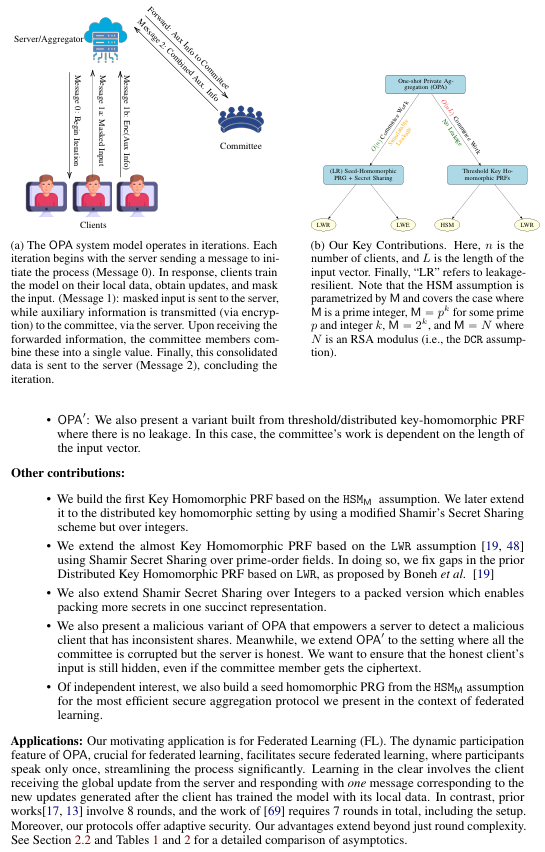
\includegraphics[
        width=2cm,
        height=2cm
    ]{structure/revision_figures/arxiv_diff_v1.png}%
};

\node[sourceimg] (papertwo)
at ($(paperone.east)+(0.95cm,0)$) {%
    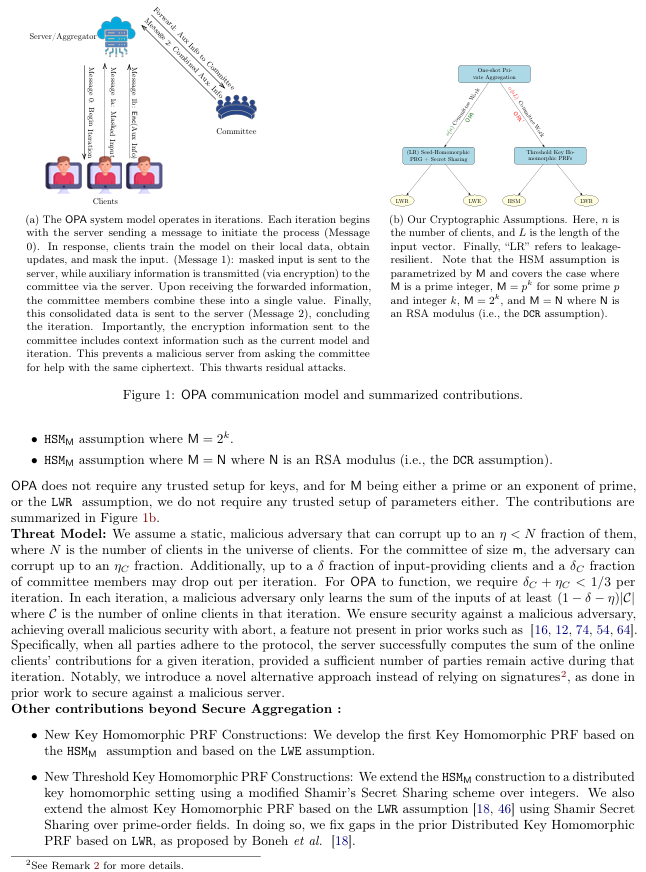
\includegraphics[
        width=2cm,
        height=2cm
    ]{structure/revision_figures/arxiv_diff_v3.png}%
};

\node[versionlabel]
at ($(paperone.north)+(0,0.0cm)$)
{$V_1$};

\node[versionlabel]
at ($(papertwo.north)+(0,0.0cm)$)
{$V_N$};

\node[dots]
at ($(paperone.east)+(0.105cm,-0.18cm)$)
{$\vdots$};

\node[
    branch,
    anchor=east,
    minimum width=1.50cm,
    minimum height=2.45cm
] (pairone)
at ($(stageone.east)+(-0.10cm,0)$) {};

\node[
    img,
    draw=red!85!black,
    line width=1.1pt
] (diffone)
at ($(pairone.center)+(0,0.70cm)$) {%
    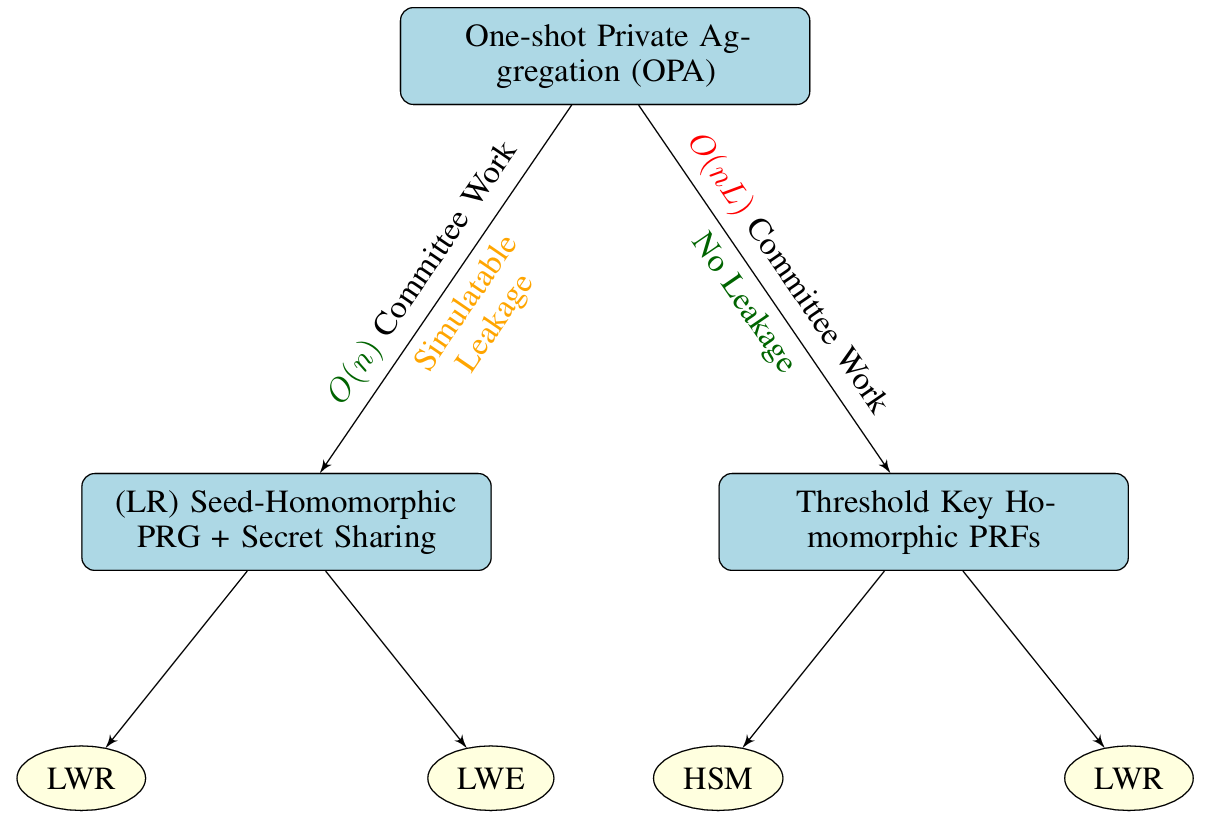
\includegraphics[
        width=1.4cm,
        height=1.4cm
    ]{structure/revision_figures/tikz_diff_v1.png}%
};

\node[
    img,
    draw=green!60!black,
    line width=1.1pt
] (difftwo)
at ($(pairone.center)+(0,-0.70cm)$) {%
    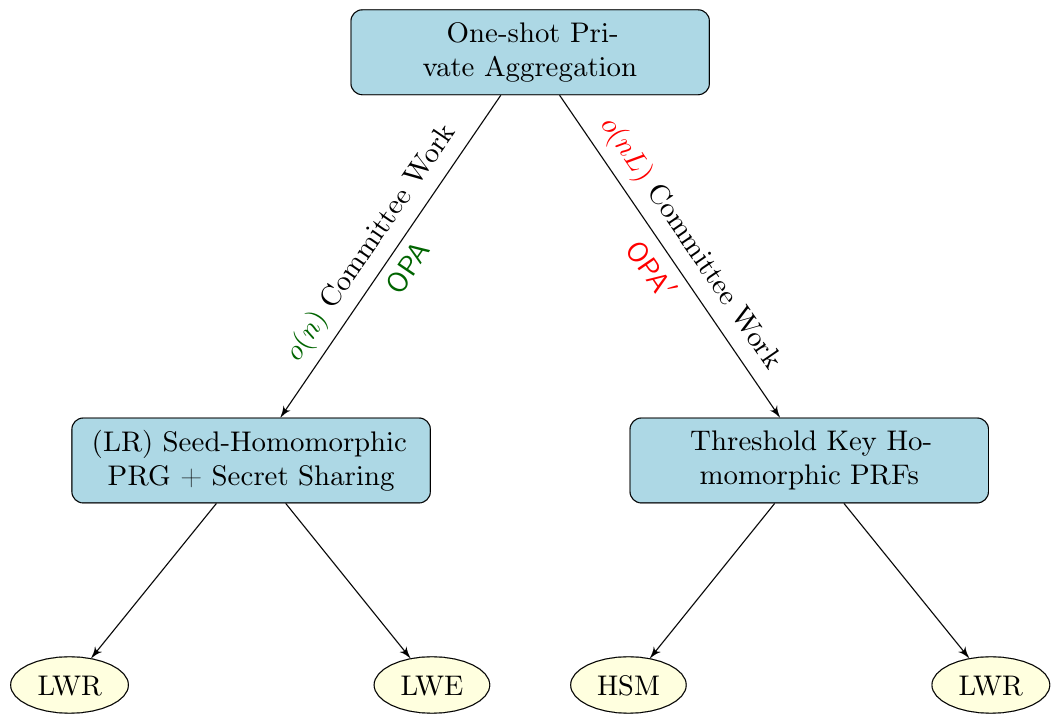
\includegraphics[
        width=1.4cm,
        height=1.4cm
    ]{structure/revision_figures/tikz_diff_v3.png}%
};

\draw[revision]
($(diffone.south)+(0,-0.03cm)$)
--
($(difftwo.north)+(0,0.03cm)$);

\coordinate (paperonefocus)
at ($(paperone.center)+(0.36cm,0.64cm)$);

\coordinate (papertwofocus)
at ($(papertwo.center)+(0.39cm,0.69cm)$);

\node[
    draw=red!85!black,
    line width=0.55pt,
    minimum width=0.55cm,
    minimum height=0.39cm,
    inner sep=0pt
] (paperonebox) at (paperonefocus) {};

\node[
    draw=green!60!black,
    line width=0.55pt,
    minimum width=0.50cm,
    minimum height=0.35cm,
    inner sep=0pt
] (papertwobox) at (papertwofocus) {};

\draw[
    red!85!black,
    ->,
    >=stealth,
    line width=0.55pt
]
(paperonebox.east)
to[out=20,in=150]
($(diffone.west)+(-0.01,0.0cm)$);

\draw[
    green!60!black,
    ->,
    >=stealth,
    line width=0.55pt
]
(papertwobox.east)
to[out=-20,in=150]
($(difftwo.west)+(-0.01,0.0cm)$);

\coordinate (redfocus)
at ($(diffone.center)+(-0.2cm,0.16cm)$);

\node[
    draw=red!85!black,
    line width=0.55pt,
    minimum width=0.27cm,
    minimum height=0.33cm,
    inner sep=0pt
] (redsource) at (redfocus) {};

\coordinate (redzoomcenter)
at ($(diffone.center)+(0.4125cm,0.121cm)$);

\begin{scope}
    \clip
        ($(redzoomcenter)+(-0.297cm,-0.363cm)$)
        rectangle
        ($(redzoomcenter)+(0.297cm,0.363cm)$);

    \node[inner sep=0pt]
    at ($(redzoomcenter)+(0.44cm,-0.352cm)$) {%
        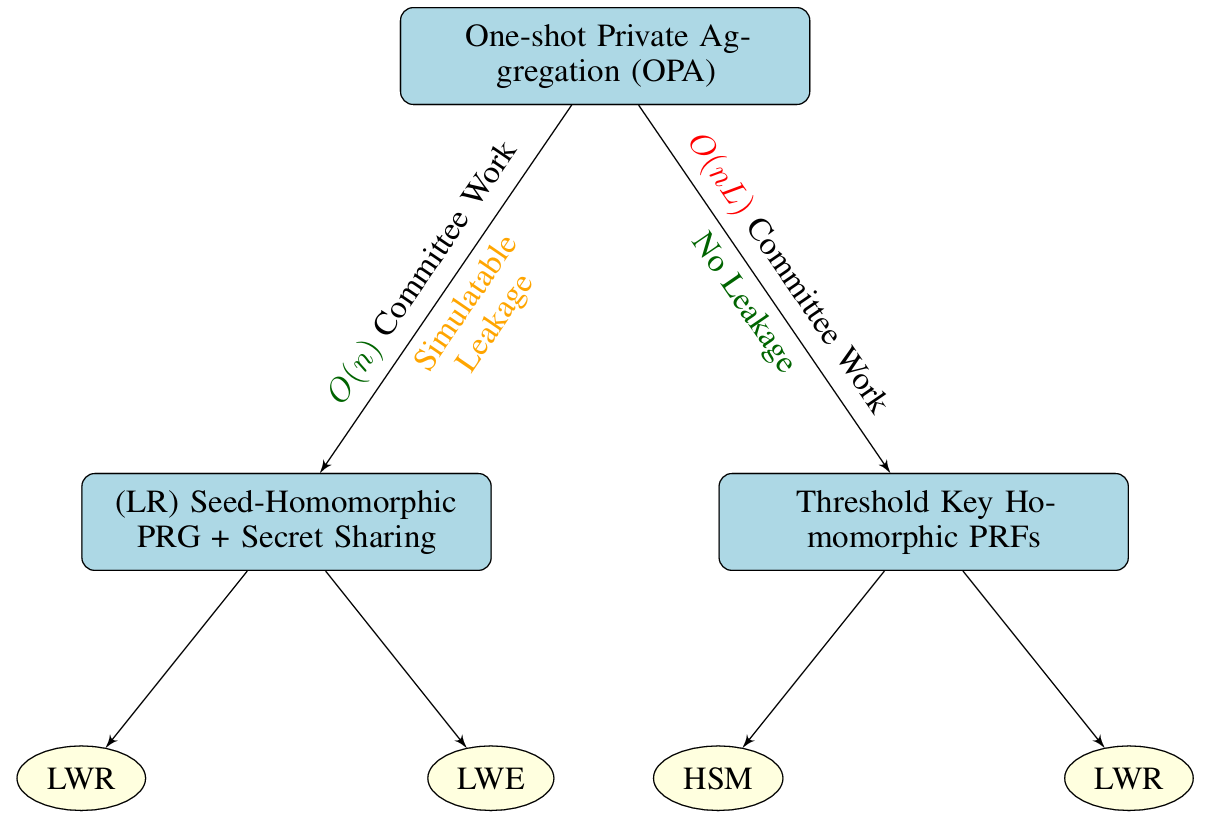
\includegraphics[
            width=3.08cm
        ]{structure/revision_figures/tikz_diff_v1.png}%
    };
\end{scope}

\draw[
    red!85!black,
    line width=0.55pt
]
($(redzoomcenter)+(-0.297cm,-0.363cm)$)
rectangle
($(redzoomcenter)+(0.297cm,0.363cm)$);

\draw[
    red!85!black,
    line width=0.45pt
]
(redsource.north east)
--
($(redzoomcenter)+(-0.297cm,0.363cm)$);

\draw[
    red!85!black,
    line width=0.45pt
]
(redsource.south east)
--
($(redzoomcenter)+(-0.297cm,-0.363cm)$);

\coordinate (greenfocus)
at ($(difftwo.center)+(-0.2cm,0.16cm)$);

\node[
    draw=green!60!black,
    line width=0.55pt,
    minimum width=0.27cm,
    minimum height=0.34cm,
    inner sep=0pt
] (greensource) at (greenfocus) {};

\coordinate (greenzoomcenter)
at ($(difftwo.center)+(0.4125cm,0.113cm)$);

\begin{scope}
    \clip
        ($(greenzoomcenter)+(-0.297cm,-0.374cm)$)
        rectangle
        ($(greenzoomcenter)+(0.297cm,0.374cm)$);

    \node[inner sep=0pt]
    at ($(greenzoomcenter)+(0.44cm,-0.352cm)$) {%
        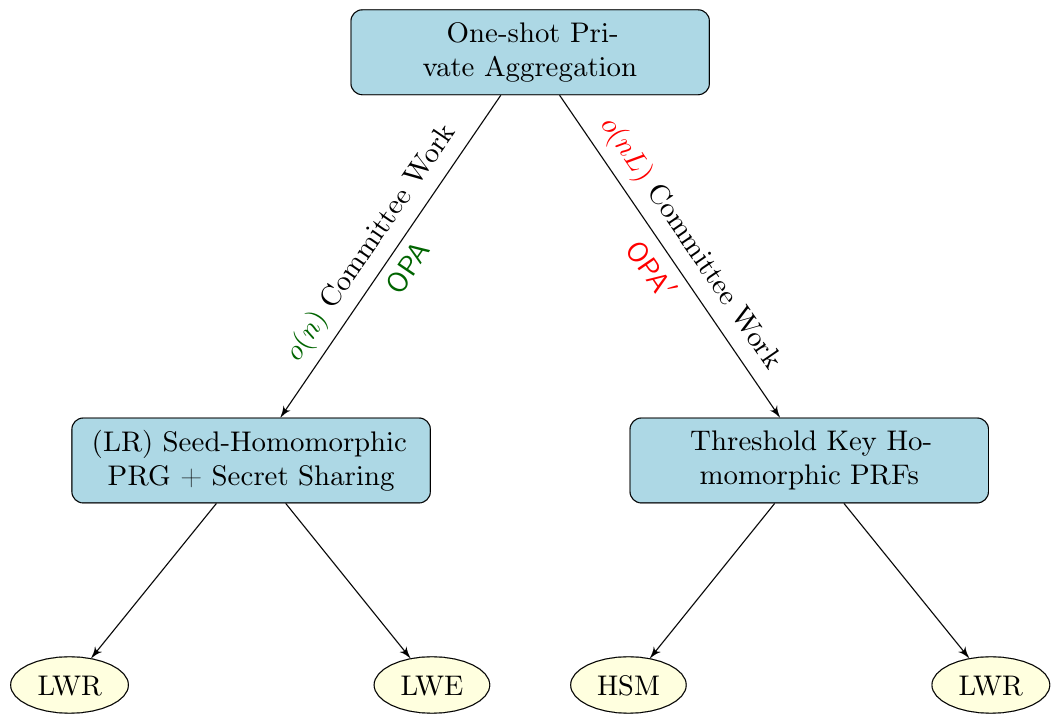
\includegraphics[
            width=3.08cm
        ]{structure/revision_figures/tikz_diff_v3.png}%
    };
\end{scope}

\draw[
    green!60!black,
    line width=0.55pt
]
($(greenzoomcenter)+(-0.297cm,-0.374cm)$)
rectangle
($(greenzoomcenter)+(0.297cm,0.374cm)$);

\draw[
    green!60!black,
    line width=0.45pt
]
(greensource.north east)
--
($(greenzoomcenter)+(-0.297cm,0.374cm)$);

\draw[
    green!60!black,
    line width=0.45pt
]
(greensource.south east)
--
($(greenzoomcenter)+(-0.297cm,-0.374cm)$);

\node[
    stage,
    anchor=south west,
    minimum width=4.75cm,
    minimum height=2.65cm
] (stagetwo)
at ($(stageone.south east)+(0.12cm,0)$) {};

\node[paneltitle]
at ($(stagetwo.north west)+(0,0.04cm)$)
{2) Related Figures/Subfigures};

\node[sourceimg] (subpaperone)
at ($(stagetwo.west)+(0.95cm,0.1cm)$) {%
    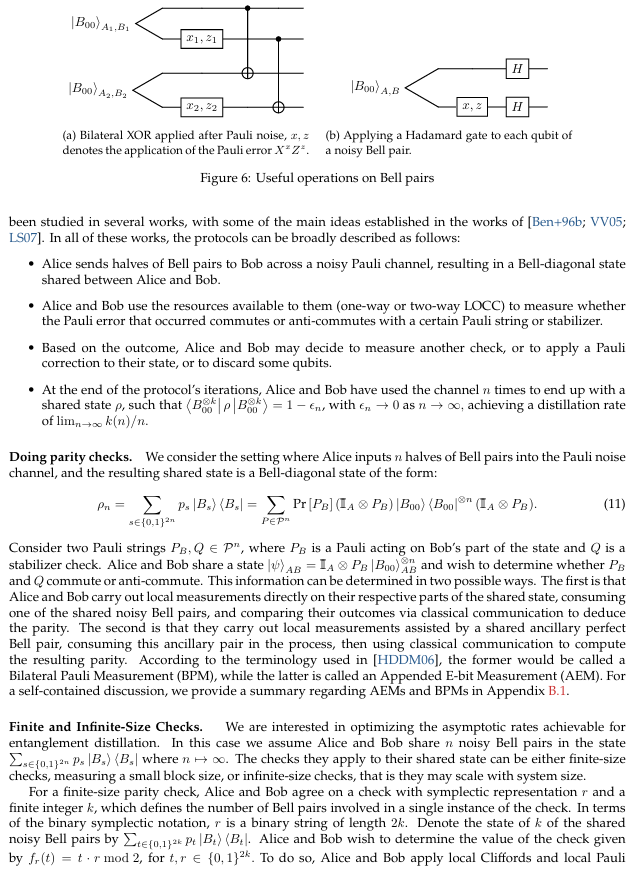
\includegraphics[
        width=2.2cm,
        height=2.2cm
    ]{structure/revision_figures/arxiv_subfigure_1.png}%
};

\node[sourceimg] (subpapertwo)
at ($(subpaperone.center)+(0.6cm,-0.2cm)$) {%
    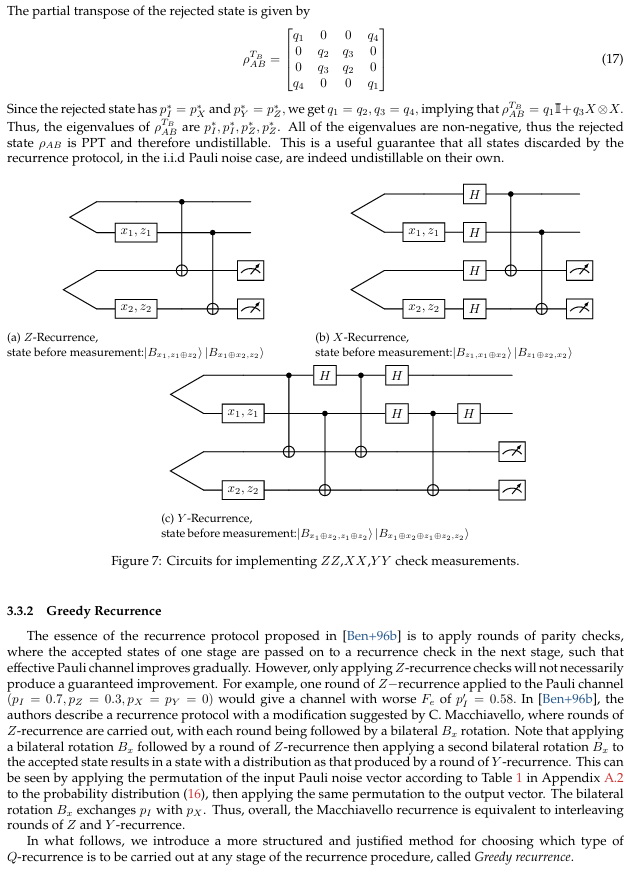
\includegraphics[
        width=2.2cm,
        height=2.2cm
    ]{structure/revision_figures/arxiv_subfigure_2.png}%
};

\node[
    branch,
    anchor=east,
    minimum width=1.9cm,
    minimum height=2.45cm
] (pairtwo)
at ($(stagetwo.east)+(-0.10cm,0)$) {};

\node[
    img,
    draw=red!85!black,
    line width=1.1pt
] (subone)
at ($(pairtwo.center)+(0,0.70cm)$) {%
    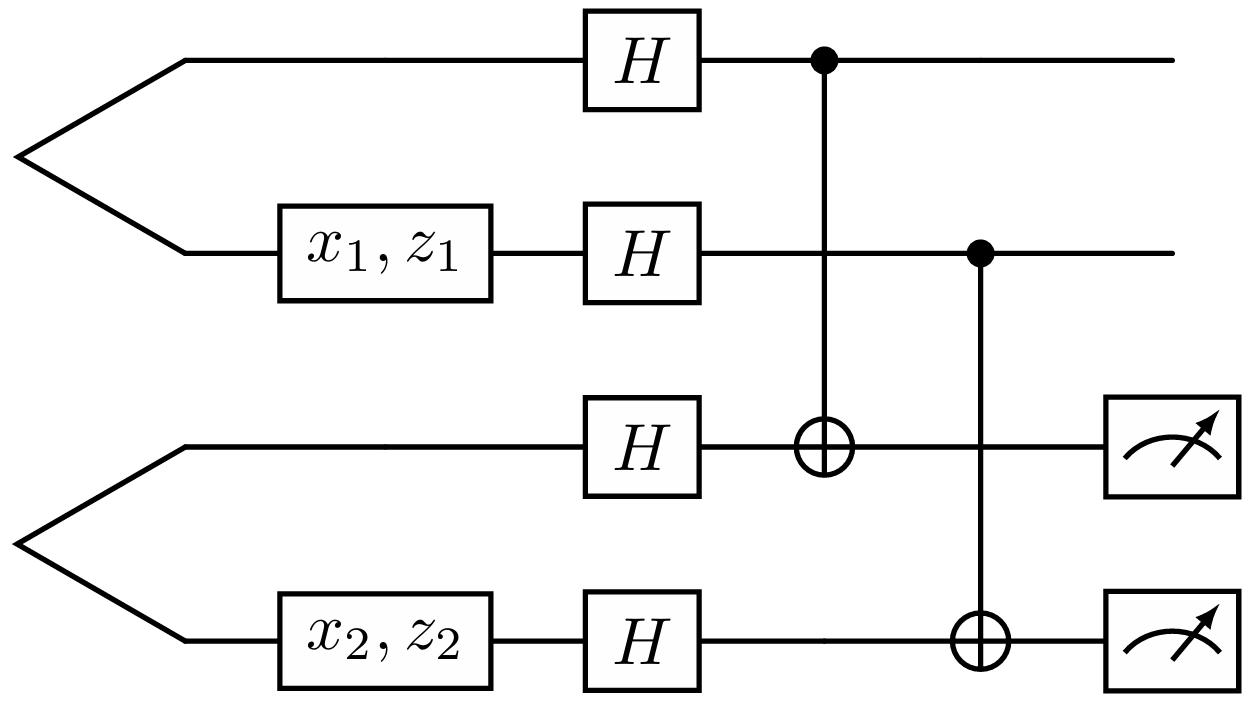
\includegraphics[
        width=1.7cm,
        height=1.7cm
    ]{structure/revision_figures/tikz_subfigure_4.png}%
};

\node[
    img,
    draw=green!60!black,
    line width=1.1pt
] (subtwo)
at ($(pairtwo.center)+(0,-0.70cm)$) {%
    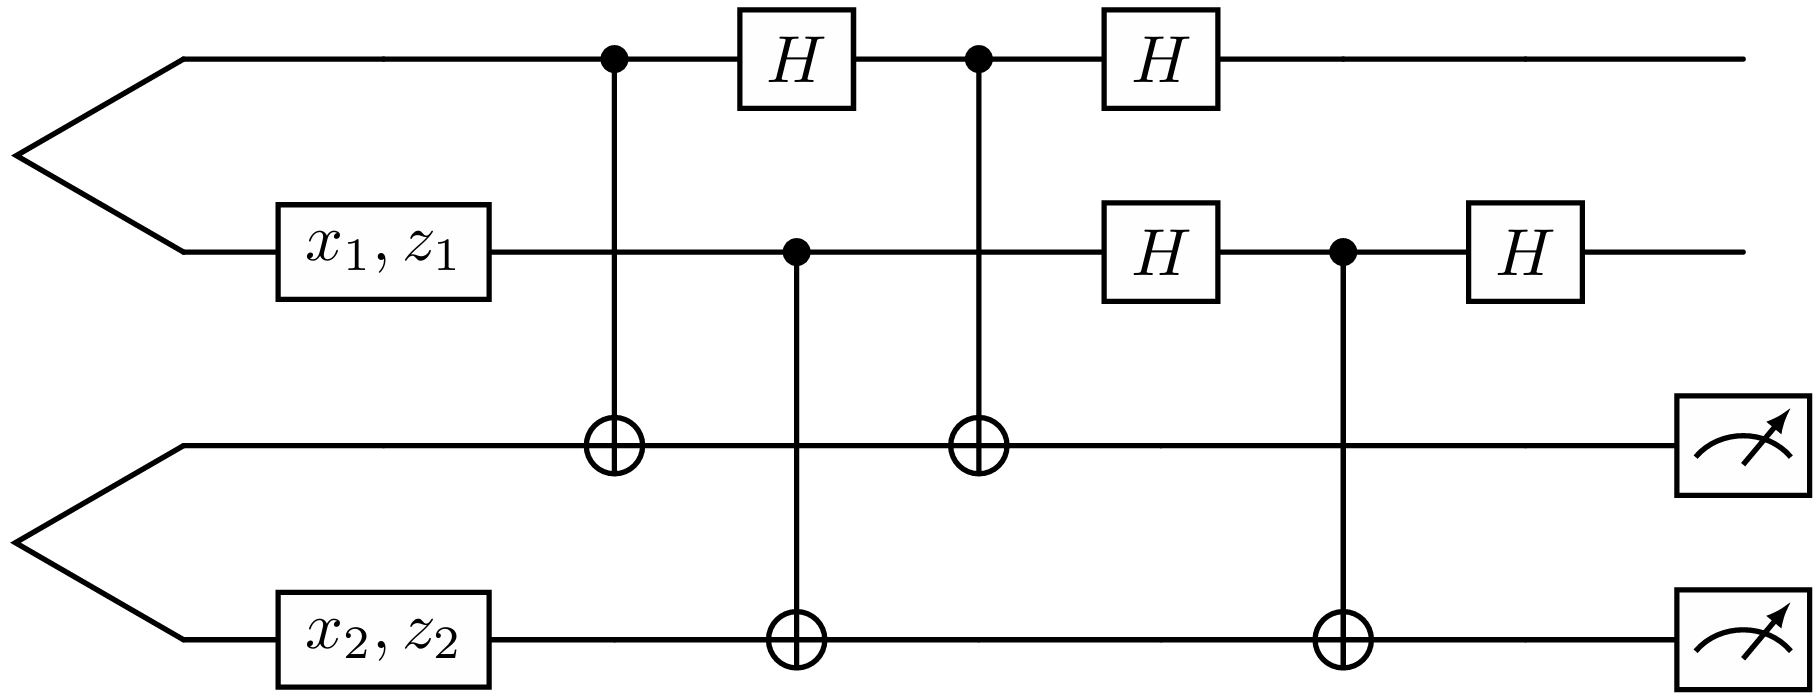
\includegraphics[
        width=1.7cm,
        height=1.7cm
    ]{structure/revision_figures/tikz_subfigure_5.png}%
};

\draw[revision]
($(subone.south)+(0,-0.03cm)$)
--
($(subtwo.north)+(0,0.03cm)$);

\coordinate (subpapertwopaironefocus)
at ($(subpapertwo.center)+(0.39cm,0.465cm)$);

\coordinate (subpapertwopairtwofocus)
at ($(subpapertwo.center)+(0.08cm,0.005cm)$);

\node[
    draw=red!85!black,
    line width=0.55pt,
    minimum width=0.645cm,
    minimum height=0.37cm,
    inner sep=0pt
] (subpapertwopaironebox) at (subpapertwopaironefocus) {};

\node[
    draw=green!60!black,
    line width=0.55pt,
    minimum width=0.93cm,
    minimum height=0.37cm,
    inner sep=0pt
] (subpapertwopairtwobox) at (subpapertwopairtwofocus) {};

\draw[
    red!85!black,
    ->,
    >=stealth,
    line width=0.55pt
]
(subpapertwopaironebox.east)
to[out=0,in=180]
($(subone.west)+(-0.01,0.0cm)$);

\draw[
    green!60!black,
    ->,
    >=stealth,
    line width=0.55pt
]
(subpapertwopairtwobox.east)
to[out=0,in=180]
($(subtwo.west)+(-0.01,0.0cm)$);

\node[
    stage,
    anchor=south west,
    minimum width=3.80cm,
    minimum height=2.65cm
] (stagethree)
at ($(stagetwo.south east)+(0.12cm,0)$) {};

\node[paneltitle]
at ($(stagethree.north west)+(0,0.04cm)$)
{3) TeX SE Discussions};

\node[sourceimg] (discussionone)
at ($(stagethree.west)+(0.8cm,0.12cm)$) {%
    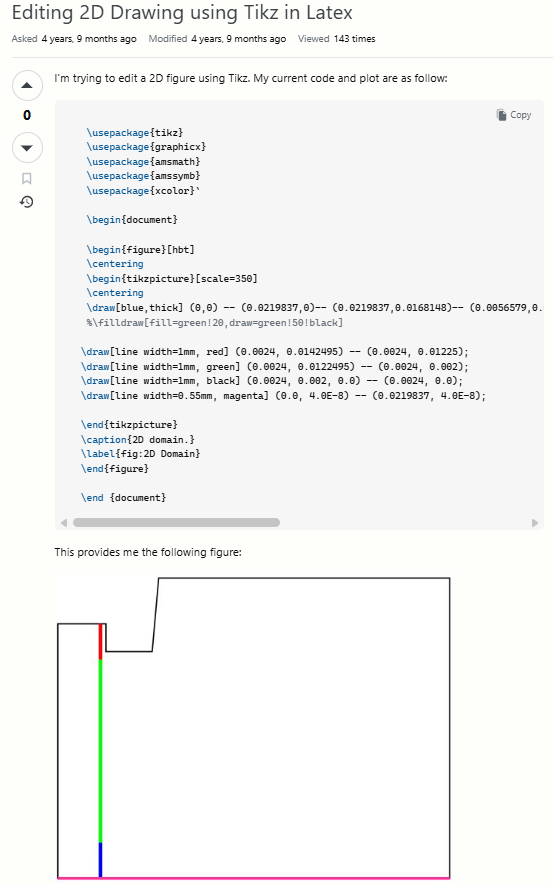
\includegraphics[
        width=2.2cm,
        height=2.2cm
    ]{structure/revision_figures/tex_discussion_1.png}%
};

\coordinate (discussiononefocus)
at ($(discussionone.center)+(0.0cm,-0.707cm)$);

\node[
    draw=red!85!black,
    line width=0.55pt,
    minimum width=1.15cm,
    minimum height=0.8cm,
    inner sep=0pt
] (discussiononebox) at (discussiononefocus) {};

\node[sourceimg] (discussiontwo)
at ($(discussionone.center)+(0.45cm,-0.24cm)$) {%
    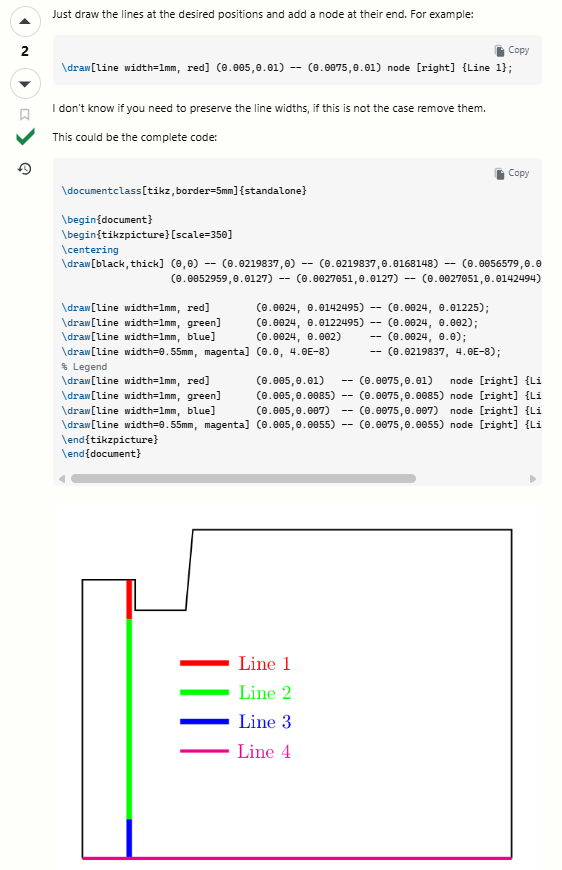
\includegraphics[
        width=2.2cm,
        height=2.2cm
    ]{structure/revision_figures/tex_discussion_3.png}%
};

\coordinate (discussiontwofocus)
at ($(discussiontwo.center)+(0.04cm,-0.655cm)$);

\node[
    draw=green!60!black,
    line width=0.55pt,
    minimum width=1.15cm,
    minimum height=0.88cm,
    inner sep=0pt
] (discussiontwobox) at (discussiontwofocus) {};

\node[
    branch,
    anchor=east,
    minimum width=1.34cm,
    minimum height=2.45cm
] (pairthree)
at ($(stagethree.east)+(-0.10cm,0)$) {};

\node[
    img,
    draw=red!85!black,
    line width=1.10pt
] (texone)
at ($(pairthree.center)+(0,0.70cm)$) {%
    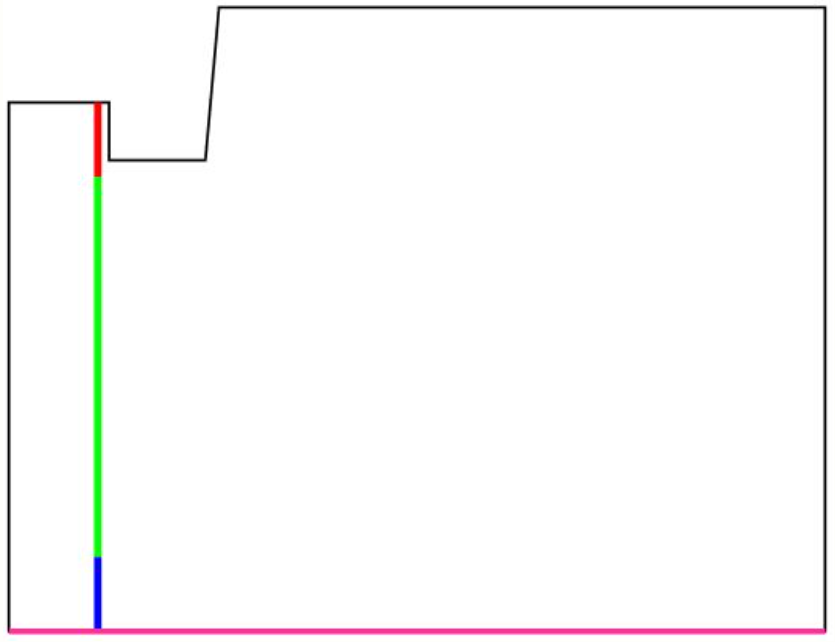
\includegraphics[
        width=1.2cm,
        height=1.2cm
    ]{structure/revision_figures/tex_tikz_1.png}%
};

\node[
    img,
    draw=green!60!black,
    line width=1.10pt
] (textwo)
at ($(pairthree.center)+(0,-0.70cm)$) {%
    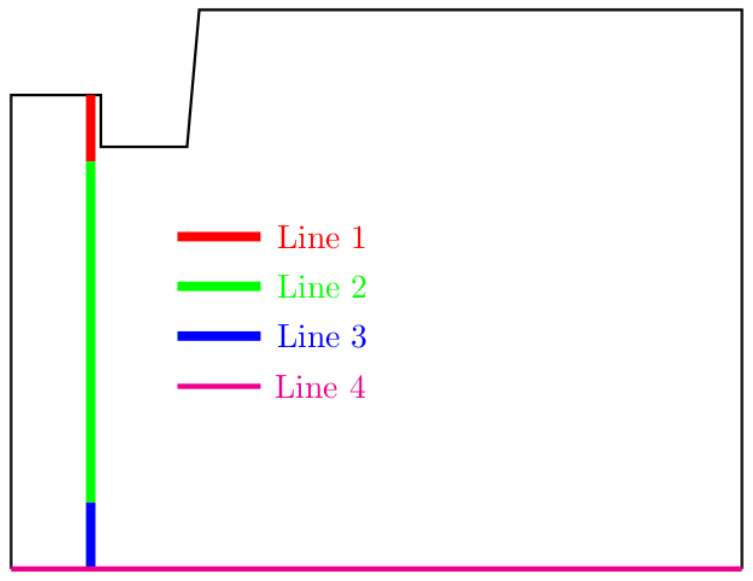
\includegraphics[
        width=1.2cm,
        height=1.2cm
    ]{structure/revision_figures/tex_tikz_2.png}%
};

\draw[revision]
($(texone.south)+(0,-0.03cm)$)
--
($(textwo.north)+(0,0.03cm)$);

\draw[
    red!85!black,
    ->,
    >=stealth,
    line width=0.55pt
]
($(discussiononebox.north)+(-0.40cm,0)$)
to[out=90,in=180]
($(texone.west)+(-0.01cm,0.0cm)$);

\draw[
    green!60!black,
    ->,
    >=stealth,
    line width=0.55pt
]
(discussiontwobox.east)
to[out=0,in=180]
($(textwo.west)+(-0.01,0.0cm)$);

\end{tikzpicture}

\caption{Sources of figure editing supervision. We recover plausible edit pairs from cross-version revisions (left), related figures and subfigures within shared scientific contexts (middle), and iterative refinements in TeX SE discussions (right). Red and green highlight paired variants in their sources.}
\label{fig:revision_sources}

\end{figure*}